% This is a comment
\documentclass[journal]{IEEEtran}
% IEEEtran.cls must be in the same folder.
% If not, manually specify the path to it like:
% \documentclass[conference]{../sty/IEEEtran}

% This is the somewhat "standard" set of packages that I typically include in all my documents. Some of them probably aren't actually used, so it isn't "pretty" but it gets the job done.
\usepackage{array}
\usepackage{url}
\usepackage{epsf}
\usepackage{verbatim}
\usepackage{morefloats}
\usepackage{flushend}
\usepackage[cmex10]{amsmath}
\usepackage{esint}
\usepackage{amssymb}
\usepackage{graphicx}
\usepackage{hhline}
\usepackage{longtable}
\usepackage{rotating}
\usepackage{lscape}
\usepackage{psfrag}
\usepackage[labelformat=simple]{subcaption}
\renewcommand\thesubfigure{(\alph{subfigure})} % makes subfigure labels appear as (a) and (b) and referenced like this in the text
\usepackage{epstopdf}
\usepackage{cite}
\usepackage{booktabs} %professional-looking tables
\usepackage{multicol} %used for getting multicolumn without page-break
\usepackage{multirow} %used for multi row in tables
\usepackage{setspace}
\usepackage[dvipsnames]{xcolor}
\usepackage{mathtools}
\usepackage{textcomp}
\newcommand{\textapprox}{\raisebox{0.5ex}{\texttildelow}} % defines a new command to make the ~ in text to denote "approximately"


% I like to keep my images that I will include as figures organized in a subfolder names "figures". 
% Adjust this appropriately for your use by either changing the path or by commenting it out if you just want to leave all the figures in the same folder as your main file.
\graphicspath{{./figures/}} 


\begin{document}
% paper title
% can use linebreaks \\ within to get better formatting as desired
% Generally good to not put math or special symbols in the title.
\title{ECE 618: LaTeX Report Template}

% I'm mashing some templates together here. If you write an actual IEEE transactions paper in LaTeX start from their template and then modify things like packages and files you want to include from there as opposed to starting from this document provided in this course.
\author{
\IEEEauthorblockN{Thomas E. Roth\IEEEauthorrefmark{2} }
\IEEEauthorblockA{\\ \IEEEauthorrefmark{2}Elmore Family School of Electrical and Computer Engineering\\
Purdue University\\
West Lafayette, Indiana 47907 \\ E-mail: rothte@purdue.edu}\\
}

% make the title area
\maketitle

% As a general rule, do not put math, special symbols or citations
% in the abstract
\begin{abstract}
Write your abstract text here.
\end{abstract}

% For peerreview papers, this IEEEtran command inserts a page break and
% creates the second title. It will be ignored for other modes.
\IEEEpeerreviewmaketitle

% the \input command allows you to tell the compiler to go through the .tex file placed in the command. Breaking out your main sections of the paper in this way helps keep the code/tex document more organized typically.
\section{Getting Started}
\label{sec:getting-started}
Before you can start using LaTeX you need to get your computer set up for it. If you don't want to go through the process of installing a few different programs on your computer, you can sign up to use Overleaf. This is an online LaTeX editor that Purdue students and faculty have access to for free. It is fairly easy to use and has nice features to enable collaborating on documents.

If you want to use LaTeX on your computer, you first need to install MiKTeX. If you google it you should be able to quickly find the download instructions. Once you have that installed, I recommend using an additional ``editor'' on top of that which has additional features to improve the usability. I personally use TeXstudio because that is what was recommended to me initially and I haven't spent any time shopping around for a different tool because it seems straightforward and capable enough.

Note that I am using the IEEE template for formatting in this document. You can easily swap to a different journal's template by substituting in their class file (replacing the IEEEtran file with something else) and making a few other edits to the main TeX document. This kind of swap can be a little tedious, but it is typically substantially easier than trying to swap between two Word document templates from different journals. I will say that the IEEE template can be a little annoying with formatting when the document you are writing only has a small amount of content in it. It usually starts to do a better job once the document gets filled in more, but if you have lots of long equations it can still struggle. These issues are why there is occasionally some weird spacing between certain sections in this document. LaTeX is doing its best to try and move things around on the pages to make it look good and match the IEEE format, but sometimes more control of these issues can be needed. I usually leave this to the editorial staff at a journal to fix, since they are going to mess with whatever you submit most of the time anyway.
\section{Introduction}
\label{sec:intro}
Rectangular cavity resonators are used in a variety of applications ranging from filters to microwave energy storage devices \cite{pozar2011microwave}. Furthermore, rectangular cavity resonators are popular due to their simplistic design which can easily be constructed by placing shorting planes on the wave ports, thereby limiting energy loss to dielectric and wall surface conductivity\cite{pozar2011microwave}. This simplistic design allows for precise control of the unloaded quality factor (Q) and resonance frequency of these resonators by simply changing material properties and cavity length for example.

All wave phenomenon in waveguides and cavity resonators for a given frequency are derivable analytically from Maxwell's Equations. Maxwell's Equations, namely Faraday's and Amp\`{e}re's laws, can describe nearly all wave interactions in electromagnetics to a level of precision that few areas in physics can match \cite{rothlecnotes}. In 1966, Kane S. Yee proposed a temporally and spatially staggered grid which could be used to explicitly solve Maxwell's Equations using finite differences in the time domain \cite{yee}. The staggered Yee grid positions the electric and magnetic fields on the edges of spatially offset voxels at half integer time-steps\cite{yee}. This method resolved many of the erroneous solutions from previous finite-difference solutions as it constructs fields able to be integrated over a line\cite{rothlecnotes} much like the integral form of Maxwell's Equations.

Finite Difference Time Domain (FDTD) is well suited to model structures as $\mathrm{TE_{10}}$ waveguides and $\mathrm{TE_{101}}$ cavity resonators due to the similarity between device length and wavelength. This length symmetry allows for relatively few spatial and temporal `points' to be used to obtain a full-wave solution in these geometries. In addition to this, FDTD facilitates the modeling of wide-band pulses allowing for results from large patches of the frequency domain to be obtained from a single simulation which is ideal for studying device resonances.
\section{Equations}
\label{sec:equations}
We can also introduce additional section structures in the following way. We can reference this section like Section \ref{sec:equations}.

\subsection{Background}
\label{subsec:background}
Here is some text within a subsection. We can reference this section like Section \ref{subsec:background}.

\subsubsection{Even Finer Background}
\label{subsubsec:finer}
We can even go to subsubsections if we want to. We can reference this section like Section \ref{subsubsec:finer}.

\subsection{Equations}
\label{subsec:equations}
Writing equations in LaTeX can be done in many ways. You can do inline equations by first typing \$ \$ and then input your math environment commands between the dollar signs. In this text within the TeX file, I had to include a backslash before the dollar sign so that LaTeX knew I wanted to actually type the dollar sign into the text and not use it to open a math environment. Now as an example of an inline equation, consider $E = mc^2$. It is a matter of practice to learn the various commands to include various mathematical operators and symbols, but many of them are fairly intuitive and can be learned quite quickly. I include here examples of a few different equations and equation environments to help you get the hang of things. In general, there are very useful online references that list out different mathematical symbols and it is usually fairly easy to ``google'' how to do just about anything you can think of in LaTeX.

We can remember that Faraday's law is
\begin{align} %align is one of the most commonly used equation environments
	\nabla\times\mathbf{E} = -\partial_t \mathbf{B} - \mathbf{M}.
	\label{eq:faraday}
\end{align}
We can reference this equation like (\ref{eq:faraday}). If we want to manually adjust the spacing between different symbols we can use the following approaches:
\begin{align} %spread things out with \,      You can do multiple of these to get more space like \,\, or \,\,\,\,\, or etc.
	\nabla \, \times \,\,\,\, \mathbf{E} = -\partial_t \mathbf{B} - \mathbf{M},
	\label{eq:faraday2}
\end{align}
\begin{align} %make things closer with \!       Same thing goes for doing multiple of these in a row
	\nabla \! \times \! \mathbf{E} = -\frac{\partial}{\partial t} \mathbf{B} - \mathbf{M}.
	\label{eq:faraday3}
\end{align}

Here are some examples of more mathematical operators:
\begin{align}
	\int_\Omega \bigg[  \big( \nabla\times\mathbf{W}\big) \cdot  \overline{\boldsymbol{\mu}}^{-1}  \cdot \big(\nabla\times\mathbf{E} \big) -   \omega^2 \mathbf{W} \cdot \overline{\boldsymbol{\epsilon}}  \cdot  \mathbf{E} \bigg] d\Omega = 0.
\end{align}
Sometimes if we have a particularly long equation we will need to spread it out over multiple lines. We can do this with
\begin{multline}  %for multiple line equations. The \\ sets where the line break should occur in the equation
	H_F = \frac{1}{2}\iiint \bigg\{ \epsilon |\mathbf{E}_q|^2 + \mu | \mathbf{H}_q|^2 + \sum_{p \in \mathcal{P}} \big[ \epsilon |\mathbf{E}_p|^2  \\ + \mu | \mathbf{H}_p|^2  \big]  - \sum_{p \in \mathcal{P}} 2 \mathbf{A}_q \cdot (\hat{n}_p\times \mathbf{H}_p ) \bigg\} d\mathbf{r}.
	\label{eq:interacting-system-hamiltonian}
\end{multline} 

We can do fancy equations that have multiple lines that we want to control how they are aligned with respect to each other in the following way:
\begin{align}
	\begin{split} % the spots in the two lines marked with the & will get aligned with each other
		\mathbf{E}(u,v,w)  &= \mathbf{E}^\mathrm{inc}(u,v,w) + \mathbf{E}^\mathrm{ref}(u,v,w)  \\
		&= E_0 \mathbf{e}_T(u,v) e^{-j \beta w} + \Gamma E_0 \mathbf{e}_T(u,v) e^{j\beta w}.
	\end{split}
	\label{eq:waveport1}
\end{align}

We can also do matrices of various types using commands like:
\begin{align}
	\overline{\boldsymbol{\Lambda}} = 
	\begin{bmatrix} %the displaystyle command makes the fraction appear in full size as opposed to getting shrunk down
		\displaystyle \frac{s_y s_z}{s_x} & 0 & 0 \\ 
		0 & \displaystyle \frac{s_z s_x}{s_y} & 0 \\
		0 & 0 & \displaystyle \frac{s_x s_y}{s_z} 
	\end{bmatrix}.
\end{align}
% t means top and the ! means to process this command right when the compiler reaches this point. 
% I had to place this here in the document so it would appear at the top of the first column rather than top of the second column and push the next figure to the next page
\begin{figure}[t!]  
	\centering
	%the command within the [] sets the width of the figure, stability-condition is the jpg name
	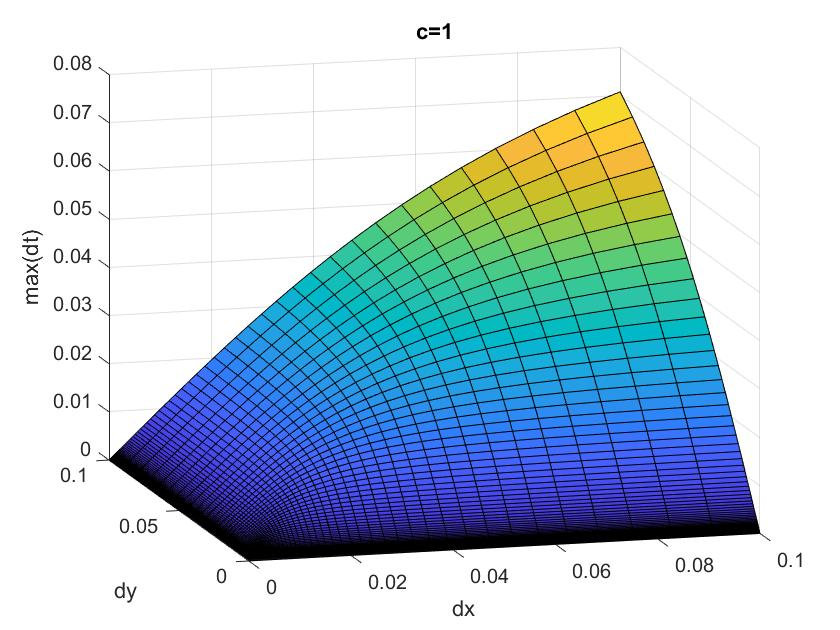
\includegraphics[width=0.9\linewidth]{stability-condition} 
	\caption{Example of caption text.}
	\label{fig:stability-condition}
\end{figure}

\section{Figures}
\label{sec:figures}
Including figures is very easy in LaTeX. It is also usually very easy to get them to appear at a desired location (e.g., the top of the page) by using simple adjustments to the figure environment. To learn more about how figures get positioned within a document (e.g., if it isn't doing what you want) you should know that they are referred to as ``floats'' in LaTeX terminology. If you google about positioning of floats in LaTeX you will likely quickly learn how you can reconfigure your TeX document to get the desired effect.

Here are some examples of how to include figures and subfigures. We can reference them like this: Fig. \ref{fig:stability-condition}, Fig. \ref{fig:waveport_ex1} is broken into two subfigures, which we can reference like Fig. \ref{subfig:waveport1} and Fig. \ref{subfig:waveport2}.

\begin{figure}[t!]
	\begin{subfigure}{0.8\linewidth} %\make this subfigure take up 80% of a linewidth
		\centering
		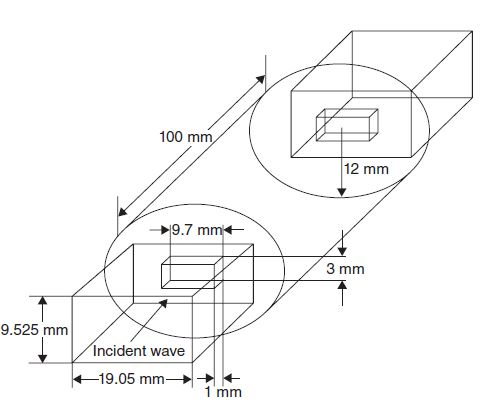
\includegraphics[width=\textwidth]{waveport1} %within this subfigure take up the entire textwidth (which was set by the linewidth command above)
		\caption{}
		\label{subfig:waveport1}
	\end{subfigure}
	\begin{subfigure}{0.9\linewidth}
		\centering
		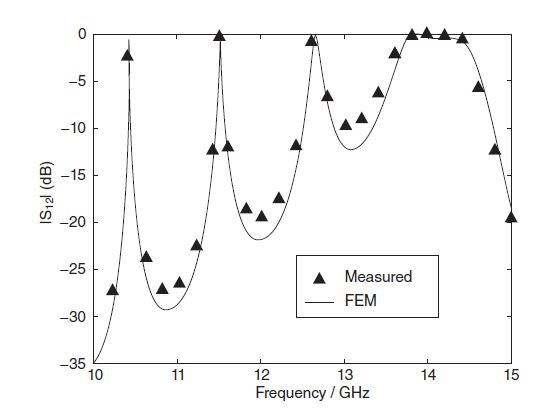
\includegraphics[width=\textwidth]{waveport2} %waveport2 is the name of the jpg file within the ./figures folder
		\caption{} %leave the caption blank, but you need the empty caption command for the (b) label to be made
		\label{subfig:waveport2}
	\end{subfigure}
	\caption{Use of wave ports to analyze a cylindrical cavity resonator. (a) The geometry analyzed and (b) the comparison of numerical and measured results (from \cite{jin2011theory}).}
	\label{fig:waveport_ex1}
\end{figure}

Here is dummy text to fill out the document to help with getting the floats positioned. The quick brown fox jumped over the lazy dog. The quick brown fox jumped over the lazy dog. The quick brown fox jumped over the lazy dog. The quick brown fox jumped over the lazy dog. The quick brown fox jumped over the lazy dog. The quick brown fox jumped over the lazy dog. The quick brown fox jumped over the lazy dog. The quick brown fox jumped over the lazy dog. The quick brown fox jumped over the lazy dog. The quick brown fox jumped over the lazy dog. The quick brown fox jumped over the lazy dog. The quick brown fox jumped over the lazy dog. The quick brown fox jumped over the lazy dog. The quick brown fox jumped over the lazy dog. The quick brown fox jumped over the lazy dog. The quick brown fox jumped over the lazy dog. The quick brown fox jumped over the lazy dog. The quick brown fox jumped over the lazy dog. The quick brown fox jumped over the lazy dog. The quick brown fox jumped over the lazy dog. The quick brown fox jumped over the lazy dog. The quick brown fox jumped over the lazy dog. The quick brown fox jumped over the lazy dog. 


\section{Reference Management}
\label{sec:reference-management}
There are various programs you can install to try and help manage your bibliography. I personally found those to be a bit annoying to use so I just maintain a BibTeX database (.bib file) for my various projects where I compile the references that I frequently use. The format to catalog all of the reference information for different BibTeX entries can be a little annoying to figure out, which is why it is rather nice that Google Scholar and some publishers directly provide the citation information in BibTeX format that you can just copy and paste into your .bib file. For instance, with Google Scholar you can search for an article, click the '' symbol below the article name and info, click the BibTeX entry at the bottom of the list, and then copy and paste what comes up into your .bib file. This usually does a pretty good job, but it will sometimes mess up certain capitalization in names/titles so it is good to check the information and edit it appropriately. You can make these edits to the .bib file within your TeX editor by opening the appropriate file. Usually, if you add a reference to your .bib file it won't appear in your auto-complete options for inserting citations until you recompile your entire document from the main TeX file. As with everything else, if you are having issues with achieving a certain effect you can typically find it answered easily via google.
\section{Conclusion}
\label{sec:conclusion}
A 3-dimensional finite difference time domain was developed from Maxwell's Equations for a rectangular waveguide and cavity resonator. The model was validated against analytic results for narrow and wide band signals thereby verifying the model's calculated fields. From this, several dielectric materials were compared for use in X-Band cavity resonators at $10$GHz. These compared results were then explained using theoretical unloaded quality factors vurther verifying the accuracy of the model.

While relatively performant, there are many optimizations that could be made to the underlying implementation. Most notably tiled approaches could be taken to improve program cache locality to alleviate the memory bound nature of the loops in this implementation. Tiled approaches would also aid in exploiting the embarrassingly parallel structure Yee's FDTD algorithm gives rise to. Further improvements could also be made to the implementation to allowing for more complex geometries to be represented which may be useful for placing devices inside waveguides or using the waveguide as a source for another device. Finally, the user experience of this implementation should be improved as it is remarkably easy to save in tens to hundreds of gigabytes of data inadvertently shifting the bottleneck away from memory to disk performance.


\bibliographystyle{IEEEtran}
\bibliography{cem_class_example_bib} %this should point to your bibliography file.

% that's all folks
\end{document}


